%%% Econ712: Macroeconomics I
%%% Fall 2020
%%% Danny Edgel
%%%
% Due on Canvas Thursday November 19th, 11:59pm Central Time
%%%

%%%
%							PREAMBLE
%%%

\documentclass{article}

%%% declare packages
\usepackage{amsmath}
\usepackage{amssymb}
\usepackage{array}
\usepackage{bm}
\usepackage{changepage}
\usepackage{centernot}
\usepackage{graphicx}
\usepackage[shortlabels]{enumitem}
\usepackage{fancyhdr}
	\fancyhf{} % sets both header and footer to nothing
	\renewcommand{\headrulewidth}{0pt}
    \rfoot{Edgel, \thepage}
    \pagestyle{fancy}
	
%%% define shortcuts for set notation
\newcommand{\N}{\mathbb{N}}
\newcommand{\Z}{\mathbb{Z}}
\newcommand{\R}{\mathbb{R}}
\newcommand{\Q}{\mathbb{Q}}
\newcommand{\lmt}{\underset{x\rightarrow\infty}{\text{lim }}}
\newcommand{\neglmt}{\underset{x\rightarrow-\infty}{\text{lim }}}
\newcommand{\zerolmt}{\underset{x\rightarrow 0}{\text{lim }}}
\newcommand{\loge}[1]{\text{ln}\left(#1\right)}
\newcommand{\usmax}[1]{\underset{#1}{\text{max }}}
\newcommand{\Mt}{M_{t+1}^t}
\newcommand{\vhat}{\hat{v}}
\newcommand{\olp}{\overline{p}}
\renewcommand{\L}{\mathcal{L}}
\newcommand{\olq}{\overline{q}}
\newcommand{\zinf}{_{t=0}^\infty}
\newcommand{\aneg}{A^{-1}}
\newcommand{\sneg}{s^{-1}}

\DeclareMathOperator{\E}{\mathbb{E}} % expected value

%%% define column vector command (from Michael Nattinger)
\newcount\colveccount
\newcommand*\colvec[1]{
        \global\colveccount#1
        \begin{pmatrix}
        \colvecnext
}
\def\colvecnext#1{
        #1
        \global\advance\colveccount-1
        \ifnum\colveccount>0
                \\
                \expandafter\colvecnext
        \else
                \end{pmatrix}
        \fi
}

%%% define function for drawing matrix augmentation lines
\newcommand\aug{\fboxsep=-\fboxrule\!\!\!\fbox{\strut}\!\!\!}

\makeatletter
\let\amsmath@bigm\bigm

\renewcommand{\bigm}[1]{%
  \ifcsname fenced@\string#1\endcsname
    \expandafter\@firstoftwo
  \else
    \expandafter\@secondoftwo
  \fi
  {\expandafter\amsmath@bigm\csname fenced@\string#1\endcsname}%
  {\amsmath@bigm#1}%
}


%________________________________________________________________%

\begin{document}

\title{	Problem Set \#2 }
\author{ 	Danny Edgel 					\\ 
			Econ 712: Macroeconomics I		\\
			Fall 2020						\\
		}
\maketitle\thispagestyle{empty}

%%%________________________________________________________________%%%

\noindent\textit{Collaborated with Sarah Bass, Emily Case, Michael Nattinger, and Alex Von Hafften}

%%%________________________________________________________________%%%
\subsection*{Question 1}

\begin{enumerate}[(a)]
	\item In a balanced growth path, households' utility and firms' profits are maximized. Thus, to find a system of equations that $C_0$, $N_0$, $w_0$, and $r_0$ must solve in a balanced growth path, we must characterize and solve the household and firm problems. To start, the household problem is given by 
		\[
			\usmax{\left\{C_t,K^s_{t+1},N^s_t\right\}_{t=0}^\infty}\sum_{t=0}^\infty \beta_t u(C_t,1-N_t)\text{ s.t. }
				\sum_{t=0}^\infty p_t\left(C_t + K_{t+1}\right) \leq \sum_{t=0}^\infty p_t\left(r_tK_t + w_tA_tN_t\right) + \pi_0
		\]
		And the firm's problem is:
		\[
			\usmax{\left\{K_t^d,N_t^d\right\}_{t=0}^\infty}\pi_0 = \sum\zinf p_t\left(Y_t-r_tK_t^d - w_tA_tN_t^d\right)\text{ s.t. } Y_t\leq F(K_t^d,A_tN_t^d)
		\]
		Where, recognizing that $\pi_0$ is monotone in $Y_t$, the firm's problem can be reduced to:
		\[
			\usmax{\left\{K_t^d,N_t^d\right\}_{t=0}^\infty}\pi_0 = \sum\zinf p_t\left(F(K_t^d,A_tN_t^d)-r_tK_t^d - w_tA_tN_t^d\right)
		\]
		Since the firm is a price-taker whose decision in each period has no bearing on its conditions in any other period, the firm's problem can be solved by solving a single arbitrary period, $t$, using first-order conditions. For all choice variables, $X$, let ${\frac{X_t}{A_t} = x_t}$:
		\[
			\usmax{\left\{k_t^d,N_t^d\right\}_{t=0}^\infty}\pi_0 = \sum\zinf A_tp_t\left(F(k_t^d,N_t^d)-r_tk_t^d - w_tN_t^d\right)
		\]
		\begin{align*}
			&K_t^d: & A_tp_tF_K(k_t^d,N_t^d) -A_tp_tr_t = 0	\\
			&		& F_K(k_t^d,N_t^d) = r_t				\\
			&N_t^d:	& p_tF_N(k_t^d,N_t^d) -p_tw_t = 0	\\
			&		& F_N(k_t^d,N_t^d) = w_t
		\end{align*}
		This solution ensures that that $\pi_0=0$. Assuming that the utility function is concave, strictly increasing, and differentiable, the constrating of the household problem holds with equality and an interior solution exists. Given the firm's solution, we can solve the constraint as:
		\[
				c_t = (r_t+1-\delta)k^s_t + w_tN^s_t - k^s_{t+1}
		\]
		Such that the household's problem has the Lagrangian function:
		\[
			\L = \sum\zinf\left[\beta^tu(A_tc_t,N_t) - p_t\lambda\left(c_t + k_{t+1} - (r_t+1-\delta)k_t - w_tN_t\right)\right]
		\]
		Which has the first-order conditions:
		\begin{align*}
			&c_t: 			& \beta^tA_tu_c(A_tc_t,N_t) = 	p_t\lambda 									\\
			&c_{t+1}:		& \beta^{t+1}A_{t+1}u_c(A_{t+1}c_{t+1},N_{t+1}) = 	p_{t+1}\lambda 			\\
			&N_t:			& -\beta^t\frac{u_N(A_tc_t,N_t)}{w_t} = p_t\lambda							\\
			&N_{t+1}:		& \beta^{t+1}\frac{-u_N(A_{t+1}c_{t+1},N_{t+1})}{w_{t+1}} = p_{t+1}\lambda	\\
			&k_{t+1}:		& \frac{p_t}{p_{t+1}} = r_{t+1} + 1 - \delta
		\end{align*}
		Where the growth of households' optimal level of consumption is dependent on wage growth:
		\[
			-u_N(A_tc_t,N_t)/w_t = A_tu_c(A_tc_t,N_t) 
		\]
		
		In equilibrium, all markets clear:
		\begin{align*}
			K_t^s &= K_t^d									&\text{(Capital)}	\\
			N_t^s &= N_t^d 									&\text{(Labor)}		\\
			C_t + K_{t+1} - (1-\delta)K_t &= F(K_t,A_tN_t)	&\text{(Goods)}
		\end{align*}
		And each initial choice variable, $N_0$ and $C_0$, and price, $w_0$ and $r_0$, satisfies the firm and household optimization conditions for a balanced growth path:
		\begin{align*}
			F_K(k_0,N_0) &= r_0									\\
			F_N(k_0,N_0) &= w_0									\\
			-\frac{u_N(A_0c_0,N_0)}{u_c(A_0c_0,N_0)} &= w_0A_0	\\
			c_0 + k_{1} - (1-\delta)K_0 &= F(k_0,N_0)
		\end{align*}
	
	\item Let $u(C,N) = \frac{C^{1-\gamma}}{1-\gamma}h(1-N)$, where $\gamma>0$, $\gamma\neq 1$. Then, the first-order conditions, provided in (a), can be used to derive:
		\begin{align}
			\beta(1+g)^{1-\gamma}\left(\frac{c_{t+1}}{c_t}\right)^{-\gamma}\left(\frac{h(1-N_{t+1})}{h(1-N_t)}\right) &= \frac{p_{t+1}}{p_t}	\\
			\beta(1+g)^{1-\gamma}\left(\frac{c_{t+1}}{c_t}\right)^{1-\gamma}\left(\frac{h'(1-N_{t+1})}{h'(1-N_t)}\right) &= \left(\frac{w_{t+1}}{w_t}\right)\left(\frac{p_{t+1}}{p_t}\right)	\\
			r_{t+1} + 1 - \delta &= \frac{p_t}{p_{t+1}}
		\end{align}
		In a balanced growth path, capital is rented at a constant $\overline{r}$. Thus, by equation (3), the price level grows at constant rate $\overline{\pi}$:
			\[
				\overline{pi} = \frac{1}{\overline{r} + 1 - \delta}
			\]
		Further, in a balanced growth path, ${N_t=N_{t+1}=\overline{N}}$. Thus, equations (1) and (2) become:
		\begin{align}
			\beta(1+g)^{1-\gamma}\left(\frac{c_{t+1}}{c_t}\right)^{-\gamma} &= \frac{1}{\overline{\pi}}	\\
			\beta(1+g)^{1-\gamma}\left(\frac{c_{t+1}}{c_t}\right)^{1-\gamma} &= \left(\frac{w_{t+1}}{w_t}\right)\left(\frac{1}{\overline{\pi}}\right)	
		\end{align}
		By (4), we can derive a constant growth rate of ${\left(\overline{\pi}\beta(1+g)^{1-\gamma}\right)^{1/\gamma}}$ for consumption and, by dividing (5) by (4), solve for the wage growth rate:
		\[
			\frac{c_{t+1}}{c_t} = \frac{w_{t+1}}{w_t}
		\]
		So consumption growth is equal to wage growth.
		
		
	\item 
	
	\item 
	
	\item 
	
	\item 
	
\end{enumerate}

%%%________________________________________________________________%%%
\subsection*{Question 2}

\begin{enumerate}[(a)]
	\item (I think this is what the state-contingent problem is)
		\[
			\usmax{\{c_t,s_t\}\zinf}\E\left[\sum\zinf\beta^t\frac{c_t^{1-\gamma}}{1-\gamma}\right]\text{ s.t. }x_{t+1}= A_ts_t\text{, }s_t\leq x_t-c_t
		\]
		The expectations operator in this case averages utility in each period across states of the world, weighting by that state's probability. Specifically, for each $t$, letting $c_t = A_{t-1}s_{t-1} - s_t$:
		\[
			\E\left[\beta^t\frac{(A_{t-1}s_{t-1} - s_t)^{1-\gamma}}{1-\gamma}\right] = \pi\left[\beta^t\frac{(A_hs_{t-1} - s_t)^{1-\gamma}}{1-\gamma}\right] + (1-\pi)\left[\beta^t\frac{(A_ls_{t-1} - s_t)^{1-\gamma}}{1-\gamma}\right] 
		\]
		
	\item In each period, the consumer's consumption-savings problem is constrained by her savings in the last period, multiplied by draw of $A$ she received that period. Thus, her relevant state variable is $A_{t-1}s_{t-1}$. The Bellman for this problem, letting $A^{-1}$ and $s^{-1}$ be the values for $A$ and $s$ in the prior period, is:
		\[
			V(A^{-1}s^{-1}) = \usmax{s}\left\{ \frac{\left(\aneg\sneg-s\right)^{1-\gamma}}{1-\gamma} + \beta\left[\pi V(A_hs) + (1-\pi)V(A_ls)\right] \right\}
		\]
		Given that $\gamma\in(0,1)$, $\frac{\left(\aneg\sneg-s\right)^{1-\gamma}}{1-\gamma}$ is clearly concave, increasing, and continuous in $\sneg$. [how do I prove this?]
	
	\item 
	
	\item 
	
\end{enumerate}

%%%________________________________________________________________%%%
\subsection*{Question 3}
To begin, we can analytically determine the steady-state of this system, which can be used to check the policy function derived by the program. Letting $\alpha$ represent the exponent on capital for Cobb-Douglas production, the Bellman of the social planner's problem is:
\[
	V(K) = \usmax{K'}\left\{\frac{\left(zK^\alpha + (1-\delta)K -K'\right)^{1-\gamma}}{1-\gamma} + \beta V(K')\right\}
\]
Taking first-order conditions and applying the envelope condition, we get:
\[
	\beta\left(z\alpha K'^{\alpha-1}+1-\delta\right)c'^{-\gamma} = c^{-\gamma}
\]
In the steady-state, $c=c'=\overline{c}$ and $K=K'=\overline{K}$, which allows us to solve:
\begin{align*}
	\overline{K} &= \left[\frac{1}{\alpha}\left(\frac{1}{\beta} + \delta - 1\right)\right]^{-\frac{1}{\alpha-1}}	\\
	\overline{c} &= z\overline{K}^\alpha - \delta\overline{K}
\end{align*}

\begin{enumerate}[(a)]
	\item The following chart displays the phase diagram for ${\Delta c=0}$ and ${\Delta K=0}$, alongside the optimal policy function, $c(K)$, which intersects the intersection of ${\Delta c=0}$ and ${\Delta K=0}$ at the steady state.
		\begin{center}
			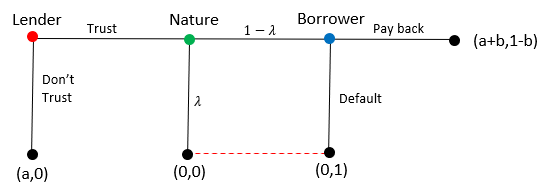
\includegraphics[scale = .8]{figure1.png}
		\end{center}
	
	\item When $\gamma$ decreases to 1.01, the steady-state values of $K$ and $c$ do not change. This is unsurprising, given that $\gamma$ does not appear in our analytical solution of the steady state. However, the saddle path gets steeper, meaning that one-time shocks will cause a larger change in consumption, and consumption will proceed to move to the steady state more quickly.
		\begin{center}
			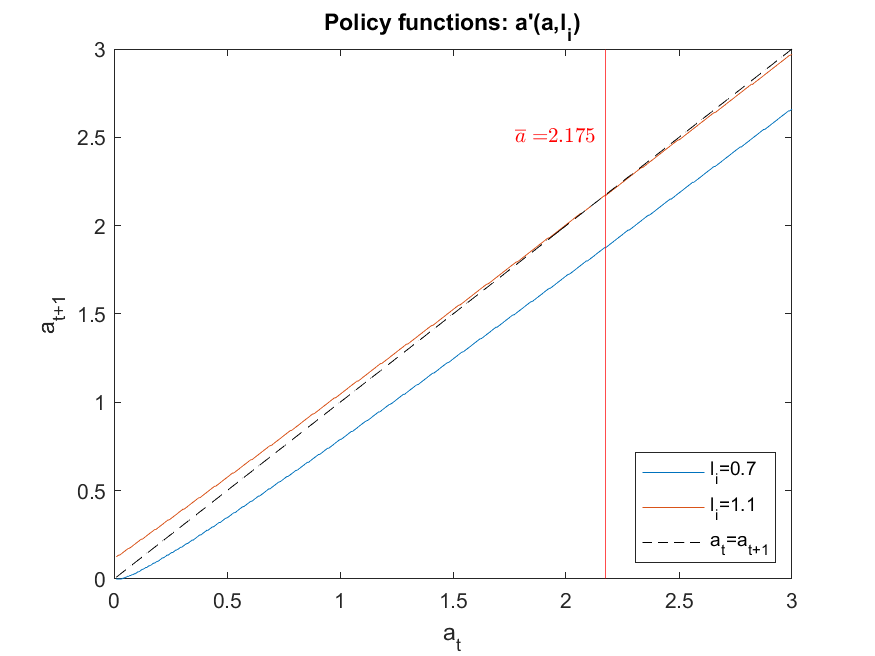
\includegraphics[scale = .8]{figure2.png}
		\end{center}
	
	\item Productivity, $z$, appears only in the steady-state value of consumption. Thus, a permanent, unexpected shock to productivity will change the steady-state value of consumption, but not that of capital. Since movements along the saddle path to the steady state are achieved by immediate changes to consumption but gradual accumulation or depreciation of capital, this shock to productivity will cause an immediate, one-time increase in consumption that moves the agent from the old steady-state to the new one. This is shown in the plot below.
		\begin{center}
			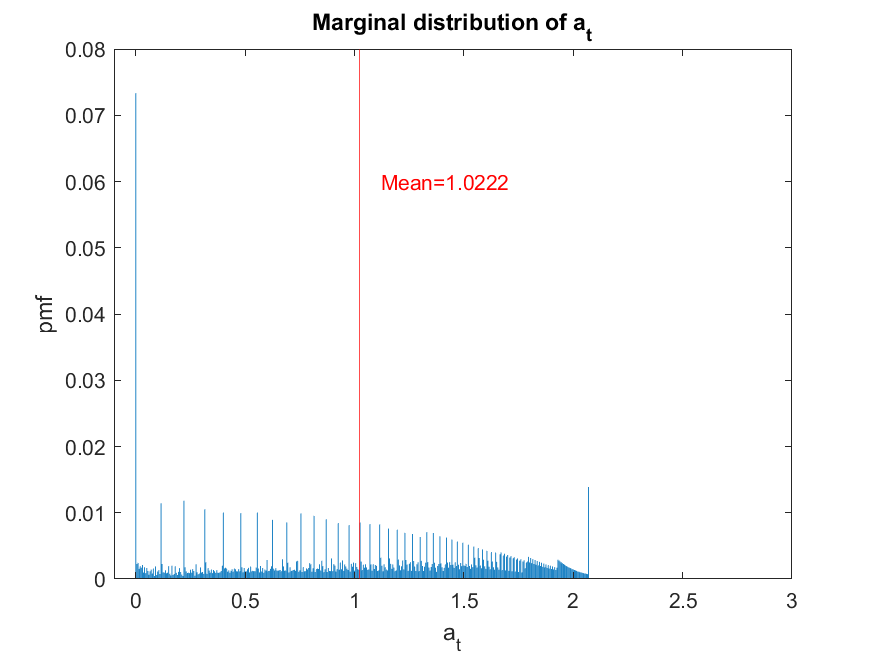
\includegraphics[scale = .8]{figure3.png}
		\end{center}
	
\end{enumerate}

%%%________________________________________________________________%%%


\end{document}












